\subsubsection{Modelo completo}

\begin{figure}[ht!]
\center
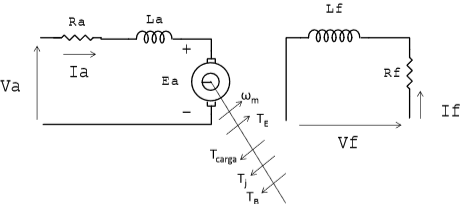
\includegraphics[scale=0.88]{imagens/circuito_31.png}
\caption{\label{fig:C31}Circuito equivalente: excitação separada, corrente de campo constante.}
\caption*{Fonte: MARTINS, cap. 2, eslaide 2.}
\end{figure}

Utilizando como base o motor com excitação separada e corrente de campo constante, como na figura \ref{fig:C31}, tem-se que, para $I_{f}$ constante,
\[V_{a} = R_{a}i_{a} + L_{a}\frac{d i_{a}}{d_{t}} + E_{a}\]
\[E_{a} = K_{e}\omega_{m}\]
\[T_{e} = K_{t}i_{a}\]
\[T_{e} = T_{carga} + J\frac{d\omega_{m}}{d_{t}} + B\omega_{m},\]
onde
\begin{itemize}
   \item $k_{e}$: Constante de velocidade.
   \item $k_{t}$: Constante de armadura.
   \item $R_{a}$, $L_{a}$: Parâmetros de armadura.
   \item B, J : Parâmetros mecânicos.
   \item J: Coeficiente de inércia.
   \item B: Coeficiente de atrito.
\end{itemize}

As equações apresentadas anteriormente modelam o motor sob qualquer alimentação de carga. Portanto, no domínio da frequência complexa,
\[V_{a}(s) = R_{a}i_{a}(s) + SL_{a}i_{a}(s) + K_{e}\omega_{m}(s)\]
\[k_{t}i_{a}(s) = T_{C}(s) + SJ\omega_{m}(s) + B\omega_{m}(s).\]
Dessa forma,
\[V_{a}(s) - k_{e}\omega_{m}(s) = (R_{a} + SL_{a})i_{a}(s)\]
\[i_{a}(s) = \frac{V_{a}(s) - k_{e}\omega_{m}(s)}{(R_{a} + SL_{a})},\]
ou também
 \[i_{a}(s) = \frac{V_{a} - k_{e}\omega_{m}(s)}{(R_{a})}\frac{1}{\left(  s + \frac{1}{\tau_{a}}\right)}.\]
 
Definindo $\tau_{a} = \frac{L_{a}}{R_{a}}$ a constante de tempo de armadura, a figura \ref{fig:D1_31} apresenta um modelo de $i_{a}(s)$ na forma de diagrama de blocos.  
 
\begin{figure}[ht!]
\center
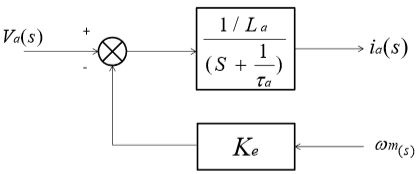
\includegraphics[scale=0.88]{imagens/diagrama1_31.png}
\caption{\label{fig:D1_31}Representação parcial em diagrama de blocos da saída em corrente.}
\caption*{Fonte: MARTINS, cap. 2, eslaide 5.}
\end{figure}

A partir da equação do torque, têm-se
\[\frac{k_{t}i_{a(S) - T_{C}(s)}}{SJ + B} = \omega_{m}(s)\]
ou
\[\omega_{m}(s) = \frac{V_{a} - k_{e}\omega_{m}(s)}{(R_{a})}\frac{1}{\left(s + \frac{1}{\tau_{a}}\right)}.\]

Sendo $\tau_{m} = \frac{J}{B}$ a constante de tempo mecânica, podemos partir da definição de $\omega_{m}$ e obter o diagrama da figura \ref{fig:D2_31}.

\begin{figure}[ht!]
\center
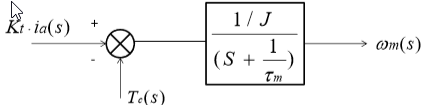
\includegraphics[scale=0.88]{imagens/diagrama2_31.png}
\caption{\label{fig:D2_31} Representação na forma de diagrama de blocos da saída em velocidade.}
\caption*{Fonte: MARTINS, cap. 2, eslaide 6.}
\end{figure}

Com os diagramas das figuras \ref{fig:D1_31} e \ref{fig:D2_31}, pode-se montar o diagrama como na figura \ref{fig:D3_31}.

\begin{figure}[ht!]
\center
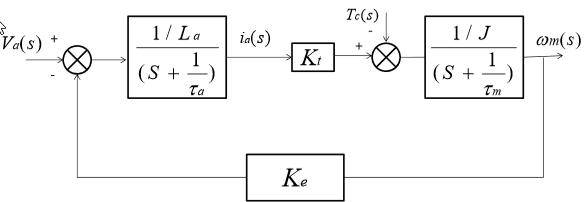
\includegraphics[scale=0.77]{imagens/diagrama3_31.png}
\caption{\label{fig:D3_31}Representação completa na forma de diagrama de blocos do motor CC.}
\caption*{Fonte: MARTINS, cap. 2, eslaide 7.}
\end{figure}

Assim, obtêm-se as funções de transferência para
\[\frac{\omega_{m}(s)}{V_{a}(s)}\]
\[\frac{i_{a}(s)}{V_{a}(s)}.\]

O sistema realimentado como na figura \ref{fig:D4_31} é caracterizado por
\[\frac{C(s)}{R(s)} = \frac{G(s)}{1  \pm G(s)H(s)}.\]

\begin{figure}[ht!]
\center
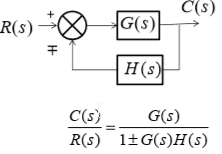
\includegraphics[scale=0.99]{imagens/diagrama4_31.png}
\caption{\label{fig:D4_31} Sistema realimentado representado na forma de diagrama de blocos.}
\caption*{Fonte: MARTINS, cap. 2, eslaide 8.}
\end{figure}

Portanto,
\[\frac{\omega_{m}(s)}{V_{a}(s)} = \frac{\frac{k_{t}}{L_{a}\left(s + \frac{1}{\tau_{a}}\right)J\left(s + \frac{1}{\tau_{m}}\right)}}{1 + \frac{k_{t}k_{e}}{L_{a}J\left(s + \frac{1}{\tau_{a}}\right)\left(s + \frac{1}{\tau_{m}}\right)}}\]

\[\frac{\omega_{m}(s)}{V_{a}(s)} =  \frac{k_{t}}{L_{a}\left[  \left(s + \frac{1}{\tau_{a}}\right)\left(s + \frac{1}{\tau_{m}}\right) + \frac{1}{\tau_{a}\tau_{ml}}\right] } .\]

Dessa forma,
\[\frac{i_{a}(s)}{V_{a}(s)} = \frac{\frac{1}{L_{a}\left(s + \frac{1}{\tau_{a}}\right)}}{1 + \frac{k_{t}k_{e}}{L_{a}J\left(s + \frac{1}{\tau_{a}}\right)\left(s + \frac{1}{\tau_{m}}\right)}},\]
i.e.,
\[\frac{i_{a}(s)}{V_{a}(s)} =  \frac{\left(s + \frac{1}{\tau_{m}}\right)}{L_{a}\left[  \left(s + \frac{1}{\tau_{a}}\right)\left(s + \frac{1}{\tau_{m}}\right) + \frac{1}{\tau_{a}\tau_{ml}}\right] } \] 
uma vez que $\tau_{ml} = \frac{R_{a}.J}{k_{e}.k_{t}}$.

\subsubsection{Modelo simplificado}

Considerando a indutância $L_{a}=0$, a configuração pode assumir a lógica do diagrama de blocos ilustrado na figura \ref{fig:D1_32} 

\begin{figure}[ht!]
\center
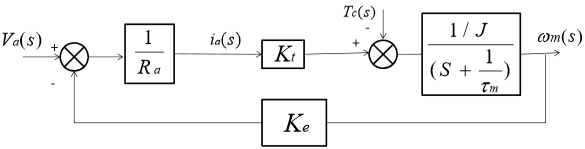
\includegraphics[scale=0.77]{imagens/diagrama1_32.png}
\caption{\label{fig:D1_32} Representação do modelo simplificado em diagrama de blocos.}
\caption*{Fonte: MARTINS, cap. 2, eslaide 10.}
\end{figure}

Dado que o torque $T_{c}$ é nulo, tem-se \[
    \frac{\omega_{m}(s)}{V_{a}(s)} = \frac{\frac{k_{t}}{R_{a}J\left(s + \frac{1}{\tau_{m}}\right)}}{1 + \frac{k_{t}k_{e}}{R_{a}J\left(s + \frac{1}{\tau_{m}}\right)}} \Rightarrow \frac{\omega_{m}(s)}{V_{a}(s)} = \frac{\frac{k_{t}}{R_{a}J}}{\left(s + \frac{1}{\tau_{m}}\right) + \frac{k_{t}k_{e}}{R_{a}J} }
\] ou
\[\frac{\omega_{m}(s)}{V_{a}(s)} = \frac{k_{t}}{R_{a}J}\frac{1}{\left[  \left(s + \frac{1}{\tau_{m}}\right) + \frac{k_{t}k_{e}}{R_{a}J}\right] }\]
\[\frac{1}{\tau_{m}} + \frac{k_{t}k_{e}}{R_{a}J} = \frac{1}{\tau_{m}} + \frac{1}{\tau_{ml}} = \frac{\tau_{m} + \tau_{ml}}{\tau_{m}\tau_{ml}} = \frac{1}{k\tau_{ml}}\]

Uma vez que $ K = \frac{\tau_{m}}{\tau_{m} + \tau_{ml}}$ 

\[\frac{\omega_{m}(s)}{V_{a}(s)} = \frac{k_{t}}{R_{a}J}\frac{1}{\left(s + \frac{1}{K\tau_{ml}}\right)} .\]

